\message{ !name(writeup.tex)}\documentclass[12pt]{article}
\usepackage[left=1in,right=1in,top=1in,bottom=1in]{geometry}
\usepackage{enumerate}
\usepackage{graphicx}
\usepackage{amsmath}
\usepackage{amssymb}
\usepackage{amsfonts}
\usepackage{amsthm}
\usepackage{enumerate}
\usepackage{url}
\usepackage{color}
\usepackage{listings}
\usepackage{wasysym}
\usepackage{tikz}
\usetikzlibrary{matrix,arrows}

\def\class{CS 5220}
\def\date{10/31/2011}
\def\prof{Professor Bindel}
\def\name{tbe4, dsj36}
\def\title{Project \#2: Smoothed Particle Hydrodynamics}
\usepackage{setspace}
\onehalfspacing

\usepackage{fancyhdr}
\pagestyle{fancy}
\lhead{\class\\\name}
\rhead{\title\\\date}

\newtheorem{lemma}{Lemma}
\def\R{\mathbb{R}}
\def\F{\mathbb{F}}
\def\C{\mathbb{C}}
\def\N{\mathbb{N}}
\def\Q{\mathbb{Q}}
\def\Z{\mathbb{Z}}
\def\C{\mathbb{C}}
\def\a{\alpha}
\def\b{\beta}
\def\d{\delta}
\def\e{\varepsilon}
\def\w{\omega}
\def\Span{\text{Span}}
\def\char{\text{char}}
\def\im{\text{im}}
\def\Hom{\text{Hom}}
\def\deg{\text{deg}}

\newcommand{\hwproblem}[2]{
\vspace{1em} \noindent{\bf #1} #2} % \vspace{1em}}
\newcommand{\hwheading}{
\thispagestyle{empty} \noindent
   \begin{center}
   \framebox{
      \vbox{
    \hbox to 5.78in { \large {\bf \class}
         \hfill \date }
       \vspace{4mm}
       \hbox to 5.78in { {\Large \hfill \title  \hfill} }
       \vspace{2mm}
       \hbox to 5.78in { \large {\it \prof \hfill \name} }
      }
   }
   \end{center}
}
\newcommand{\hwsolution}[1]{\vspace{1em} \noindent {\emph{#1.}}}

\lstset{
  basicstyle=\footnotesize,
  language=C,
  frame=single
}

\def\ind{\vspace{0.75em}\noindent}

\begin{document} \hwheading

\message{ !name(writeup.tex) !offset(-3) }
 \hwheading

\subsection*{Introduction}
Our project involved optimizing a smoothed particle hydrodynamics
simulation. We started with a reference serial implementation and
made two salient improvements: improving the asymptotic complexity
of the simulation by employing spatial partitioning and parallelizing
the codes. We used OpenMP for this project, as suggested, which
allows easy management of shared memory. However, to get the code
to run fast, we had to restructure a good amount of our computations
to prevent the different threads from ``stepping on each other's
toes,'' so to speak.

\subsection*{Spatial Partitioning}
For each particle, the SPH simulator computes an interaction with
all of the particles within some fixed radius $h$ of the particle.
This search is done for both the density and acceleration computations.
The reference code used a brute force search on the particles for
each particle's computation, yielding $O(n^2)$ complexity. As suggested,
we used a form of spatial binning to improve this complexity to roughly
$O(n)$.

\ind Our approach is as follows. First, to improve locality, we store
the particles as structures, with each containing its position, acceleration,
and so forth. The reference implementation stored each attribute in a
global array, so accessing the different attributes for a single
particle would require looking though many different arrays. Furthermore,
each particle structure has a pointer to a next particle, allowing us
to create linked lists of particles easily. Using this addition, we include
an array of pointers to particles (so, in essence, an array of linked
lists of particles) in the state structure. These linked lists are the
``bins'' in our optimization.

\ind The first order of business is to decide how many bins to have in
our simulation. It is very desirable to have bins of width no less than
$2h$, as this property guarantees that any circle of radius $h$ within
a bin can only touch at most three neighboring bins. On the other hand,
we do not want a large number of particles in a single bin, as search
through a bin is necessarily linear. Therefore, we compute an estimate
for the number of bins where there is, on average, one particle per
bin. We then take the larger of the two bounds.

\ind Once the bins have been set up, the next step is to insert the particles
into the bins. The strength of our data structure is that deciding which
bin a particle should live in is $O(1)$, implying that inserting all
the particles is $O(n)$. Since we know the height and width of the
bins, computing which bin is simply a matter of dividing the coordinates
of the particle by the dimensions of the bin and taking the floor.
Once we know which bin a particle should go into, insertion into a
linked list is just $O(1)$ as well.

\ind Now that we have the particles in their bins, we can speed up the
density and acceleration computations significantly. For each particle,
we receive at most four linked lists of bins from our {\tt get\_neighboring\_bins}
function. This function considers the circle of radius $h$ around the
point and returns all of the bins that intersect this circle. We
may then search this subset of the particles in the usual fashion,
adding the contributions of particles that are within $h$ of our
fixed particle. We use this optimization in the {\tt compute\_density}
and {\tt compute\_accel} functions.

\ind Although our approach described so far improves the quadratic
brute force search, following the next pointers in each bin's
linked list may cause our simulation to have very poor cache
locality. This poor cache performance is due to there being no
inherent relationship between a particle's place in the state structure's
particle array and its bin. Thus, we sort the particles after every
200 iterations or so to move particles in the same bin close to each
other in memory. As suggested, we used a linear time bucket
sort to rearrange the particles.

\subsection*{Parallelization and Symmetry}
After adding binning to our simulation, we next turned our focus to
parallelizing the codes. Parallelizing the leapfrog integrator was
trivial, as there are no data dependencies between the particles
in that stage. Therefore, we simply added a {\tt \#pragma omp for},
which evenly splits the work for that loop over the threads.

\ind The first optimization we made for the interaction functions
was to use the symmetry inherent in the model to halve the amount
of work done. The density and acceleration contributions from particle
$i$ to particle $j$ are identically the contributions from particle
$j$ to particle $i$. Therefore, we may update them both in
one step, halving the number of particle pairs we need to consider.
To make sure we do not update a pair twice, we simply keep a flag
on each particle indicating whether it has been seen already. If
the second particle in a potential interaction has been seen
already, the pair has already been computed.

\ind Parallelizing this idea is not immediately straightforward,
as expected. Our idea is split the columns of bins evenly among
the threads. However, each column of bins, with this symmetry handling
added, needs to write to itself, the column to the left, and the column
to the right. If two threads are simultaneously handling adjacent
columns, they may both try to write to the same particle, causing
blocking or, at worst, a race condition. Our solution to this problem
is to make three passes over the bins. We do every third column in
each pass, leaving two columns between any column being worked on.
This pattern means that each thread can write to the column around without
fear of race conditions or requiring a lock.

\subsection*{Performance}
First, we will analyze the performance of our binning optimization.
As expected, using our improved version significantly improved performance,
and the collected data suggests that our asymptotic behavior has indeed
changed from quadratic to linear.

\begin{figure}[h!]
  \centering
  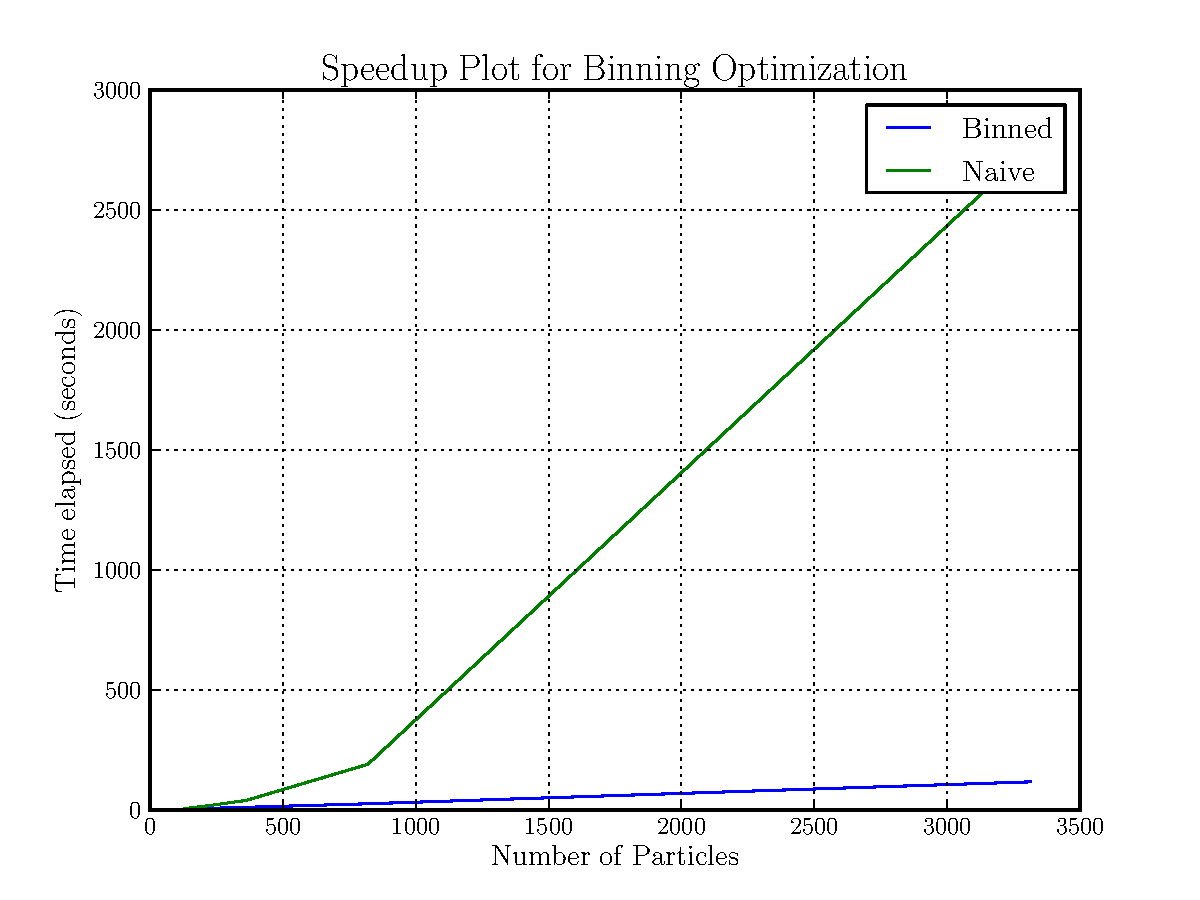
\includegraphics[scale=0.5]{bin_speedup.pdf}
\end{figure}



\end{document}

\message{ !name(writeup.tex) !offset(-195) }
